\documentclass{article}
\usepackage[lmargin=3cm, tmargin=3cm, rmargin=2cm, bmargin=2cm]{geometry}
\usepackage[onehalfspacing]{setspace}
\usepackage[utf8]{inputenc}
\usepackage[T1]{fontenc}
\usepackage[brazil]{babel}
\usepackage{amsmath, bbm}
\usepackage{graphicx, graphics, xcolor, comment, enumerate, multirow, multicol, indentfirst}
\usepackage{hyperref}
\usepackage{float}
\usepackage{setspace} \doublespacing 

\title{MAP2212 - EP4 Estimativa de uma integral com base em geradores randômicos não-uniformes}
\author{Vinícius da Costa Collaço - 11811012 \and Nikolas Lukin - 5381328}

\renewcommand*\contentsname{Sumário}
\renewcommand\refname{Referências}

\begin{document}
\setlength{\parindent}{1cm} 
\maketitle
\begin{center}
\Large{Instituto de Matemática e Estatística}\\
\Large{Universidade de São Paulo}\\
\begin{figure}[htp]
  \centering
  
\includegraphics[scale=1]{Imagens/IME.jpg}
  \label{fig:IME}
\end{figure}
\Large{Maio de 2022}
\end{center}
\pagebreak
\tableofcontents
\pagebreak

\maketitle

\section{Introdução}

Esse relatório visa apresentar uma solução para o quarto exercício programa (EP4) proposto na matéria MAP2212/2022 (Laboratório de Computação e Simulação) do curso de bacharelado de matemática aplicada e computacional (BMAC) do instituito IME-USP.\\
O objetivo deste EP é estimar a função verdade definida por,
\begin{equation}
    W(v)= \int_{T(v)} f(\theta\mid x,y)d\theta 
\end{equation}
através de uma função \textit{U(v)} obtida por integral condensada da massa de probabilidade\cite{kaplan1987improved} de $f(\theta|x,y)$ no domínio \textit {T(v)} e que não ultrapassa um nível \textit{v} pré-estabelecido, ou seja,
\begin{equation}
    T(v)=\{ \theta  \in   \Theta  \mid f(\theta\mid x,y)\leq v\}
\end{equation}
A função \textit{f} é a função de densidade de probabilidade posterior de \textit{Dirichlet}, que representa um modelo estatístico m-dimensional multinomial, dado por:
\begin{equation}
    f(\theta\mid x,y) =  \frac{1}{B(x+y)}  \prod_{i=1}^m  \theta_i^{x_i+y_i-1} 
\end{equation}
onde \textit{x} é um vetor de observações, \textit{y} é um vetor de observações a priori, $\theta$ é um vetor simplex de probabilidades, \textit{m} = 3 é a dimensão e \textit{B} representa a distribuição Beta. Observe que, 
\begin{equation}
    x,y \in   \aleph ^m,  \theta  \in  \Theta =S_m=\{ \theta  \in  \Re _m^+ \mid f(\theta\mid x,y)\leq v\}
\end{equation}
Nas próximas seções demonstraremos como estimamos a função verdade usando integral condensada e a variante de geradores randômicos não-uniformes,
Utilizando a linguagem \textit{Python} e bibliotecas adequadas\cite{harris2020array, Waskom2021, Hunter:2007, 2020SciPy-NMeth}, 

\section{Definindo o tamanho do n}

Para a definição do valor do n, iremos utilizar a aproximação assintótica de uma distribuição Bernoulli para determinar a quantidade de pontos dentro de um bin necessários para satisfazer a resolução e o erro máximo tolerável definido em $\epsilon = 0.05\% $. A quantidade \textit{k} de bins deve ser tal a garantir uma resolução que seja maior que o erro $\epsilon$,

\begin{equation}
    W(v_j) - W(v_{j-1}) = \frac{1}{k} \geq \epsilon
    \label{eqn:valork}
\end{equation}

Supondo que o tamanho da amostra seja relativamente grande, pelo teorema do limite central, podemos aproximar a Bernoulli por uma normal, tendo:

\[
P(|\hat{p} - p|\leq \varepsilon)\geq \gamma 
\] \cite{estatbas}

\[
P(-\varepsilon \leq \hat{p} - p \leq \varepsilon) = P\left( \frac{-\sqrt{n}\varepsilon}{\sigma} \leq Z \leq \frac{\sqrt{n}\varepsilon}{\sigma}\right) \approx \gamma
\]
obtendo finalmente 

\begin{equation}
    n = \frac {\sigma^2 {Z_\gamma}^2} {\varepsilon^2}
    \label{eqn:valorn}
\end{equation}

esse resultado obtido em \ref{eqn:valorn} será utilizado para definir o número de pontos necessários para resultar no erro mínimo exigido. 

\subsection{Número de bins (k)}

O número de bins da distribuição discreta de probabilidades deve ser tal que permita uma resolução maior que o erro estipulado, definido em \ref{eqn:valork}

\begin{equation}
    k \geq \frac{1}{\epsilon} \implies k \geq 2000
    \label{eqn:valork}
\end{equation}

Para uma resolução melhorada no programa foi utilizado 
\begin{equation*}
    k = 4000
\end{equation*}

\subsection{Intervalo de confiança}

Para o problema será utilizado um intervalo de confiança $\gamma = 95\%$, escolhido arbitrariamente obtendo assim o $Z_\gamma$ da $N(0,1)$, portanto $Z_\gamma = 1,96$.

\subsection{Erro $(\varepsilon)$}

Para o cálculo do n será utilizado o valor do erro relativo exigido entre o valor real de $W(u)$ e sua estimativa, portanto $\varepsilon = 0,0005$

\subsection{Variância amostral}

Para o cálculo da variância, considera-se que os pontos se distribuem segundo uma distribuição de Bernoulli dentro de um bin com probabilidade igual à resolução do bin. Com o valor de $k = 4000$ variância pode ser determinada por,

\begin{equation}
    \sigma^2 = \frac{\epsilon}{2} (1 - \frac{\epsilon}{2}) \approx \frac{\epsilon}{2}
    \label{eqn:valorsig}
\end{equation}

\subsection{Valor final do n}

O cálculo do n pode ser obtido através das equações em \ref{eqn:valork} \ref{eqn:valorn} \ref{eqn:valorsig} resultando em,

\begin{equation*}
    n = k \cdot \frac{1,96^2\cdot \frac{\epsilon}{2}}{\epsilon^2} \geq 15.366.400
\end{equation*}

portanto:

\[
    n_{min} = 15.366.400 \ pontos
\]

\section{Resultados e discussão}

Para a simulação construiu-se um algoritmo que recebe como dados de entrada os vetores \textit{x} e \textit{y}, constrói e ordena crescentemente uma lista com \textit{n} entradas de $f(\theta|x,y)$ obtidas de simulações aleatórias de $\theta_i$ advindas de um gerador gerador randômico não-uniforme (Gamma). Esta lista é condensada em uma lista menor com \textit{k} bins, os quais cada um condensa a informação de  \textit{n/k} pontos. Finalmente, o algoritmo percorre esta última lista e localiza a posição \textit{i} correspondente ao cut-off \textit{v}. O valor calculado da integral condensada \textit{U(v)} é obtido por,

\begin{equation}
    \left\{\begin{matrix}
    U(v)= 0, & v \leq min(f(\theta\mid x,y))\\ 
    U(v)= \frac{i}{n} & min(f(\theta\mid x,y)) \leq v \leq max(f(\theta\mid x,y))\\ 
    U(v)= 1, & v \geq max(f(\theta\mid x,y))
    \end{matrix}\right.
\end{equation}
\linebreak
O gráfico de \textit{U(v)} está ilustrado na Figura \ref{fig:int} e a Tabela \ref{tab:validation} resume alguns valores de \textit{W(v)} fornecidos pelo monitor para validação dos resultados.

\begin{figure}[htp]
  \centering
  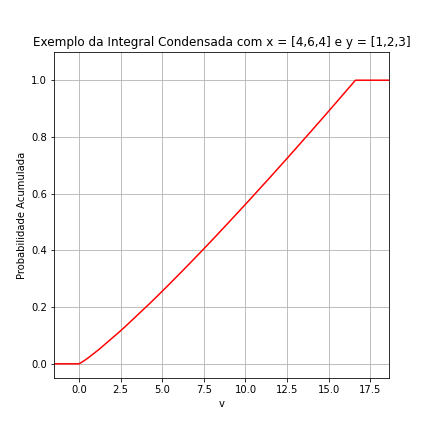
\includegraphics[scale=0.85]{Imagens/Integral.png}
  \caption{Gráfico de \textit{U(v)}}
  \label{fig:int}
\end{figure}

\begin{table}[h!]
\centering
 \begin{tabular}{||c c c c||} 
 \hline
 v & W(v) & U(v) & Erro (\%) \\ [0.5ex] 
 \hline\hline
 0.00 & 0.00 & 0.00 & 0 \\ 
 0.50 & 0.02 & 0.02 & 0 \\
 1.00 & 0.04 & 0.04 & 0 \\
 15.0 & 0.89 & 0.89 & 0 \\
 500 & 1.00 & 1.00 & 0 \\ [1ex] 
 \hline
 \end{tabular}
 \caption{Validação de \textit{U(v)}}
 \label{tab:validation}
\end{table}

\section{Conclusão}

Com os resultados obtidos no trabalho, foi observado um método efetivo para o cálculo da integral da função verdade através da discretização da distribuição de \textit{Dirichlet} usando geradores randômicos não-uniformes implementado em Python. 

O algoritmo implementado mostrou-se eficiente para cálculos de diversos \textit{U(v)} após a implementação da classe, cumprindo assim os requisitos exigidos pelo problema proposto.

\newpage
\bibliographystyle{plain}
\bibliography{ref.bib}

\end{document}
